\chapter{Introduction}
% 1. general introduction
This thesis describes the design and implementation of an efficient, high-speed
TCP/IP network stack intended to run on custom hardware where performance, responsiveness,
and throughput is crucial.\\

% 2. Explanation of specific problem
As is the trend with modern automation, computerization, and mechanization, new
devices are steadily invented to handle this increasing demand for data and
control.
With the ever-increasing sophistication of machines generating immense amount
of information, the data needs to be transmitted to numerous other machines for
further processing, or even simply storage. The most common and the most convenient
way of linking multiple devices together is using the internet, and its underlying
protocols. However, the networking stack supplied with most major operating
systems, while heavily optimised, suffers from considerable penalties due to
complexities of a standard computer architecture. For example, heavy network
traffic utilizes the computers' internal busses, utilizes the memory, and spend
precious \gls{cpu} clock-cycles with polling and interrupts. This
prevents the machine from using these resources for other computing tasks.\\
These issues have been identified and solved by hardware manufacturers by
adopting dedicated \gls{nic}, which would employ
various techniques to offload the processing. One such offloading technique is
called the \gls{toe}, which usually takes care of the essential
parts of networking involved -- the \gls{ip} and the \gls{tcp}\cite{TCP_offload_dumb_idea}.\\
Modern hardware manufacturers can produce NICs boasting network throughput
speeds as high as 100 Gigabits\cite{xilinx_100g_nic}. Unfortunately, these cards
are highly specialized for certain applications, and even though they provide
basic programmability, they are rarely suitable for rapid prototyping of
applications and other custom hardware devices. Furthermore, each NIC manufacturer
has a diverse set of hardware with varying interfaces, making it hard to
combine, swap and test these cards.
Licensed software solutions in the form of IP blocks exist as well
\cite{microtronix_ip_cores}\cite{avnet_ip_cores}. Unfortunately,
these blocks are usually distributed as black-boxes of \gls{vhdl}
code, which is hard to maintain, and even harder to debug and
extend\cite{opencores_mission}.  Additionally, these IP blocks or
"cores" are exceptionaly expensive for smaller design teams, making
it nearly impossible to prototype hardware designs with limited
funding\cite{opencores_mission}. Multiple networking IP cores exist gratis for
non-commercial use, but use for these is very limited by that nature.
Buying a licence for such IP cores is not an easy task either, as the
prices of the licences are rarely listed on the vendor sites, and the
sales departments have to be contacted for a custom quotation. It is
also common to either require a lawyer to verify and sign the excessive
license agreements, or having to sign up for memberships of various
IP Licensing deals, such as the SignOnce IP Licensing program by
Xilinx\cite{xilinx_signonce}.\\

In this thesis, we bridge the gap between the blazingly-fast network offloading
devices and their more flexible and malleable software counterparts.\\
This networking stack is implemented in a fully self-contained fashion so that
it is completely independent of any other software running on the machine, while
utilizing the performance advantages gained from the lack of overhead in
conventional implementations.
The use of a high-level programming language in combination with the modern
\gls{sme} model makes the network stack a very versatile
implementation with ease of use, debugging, and even extension.


\section{Related work}
Networking is indeed desired in more and more applications and hardware devices.
As a consequence, there exist projects that bring the internet protocol suite to
the FPGA hardware. One such project is the Xilinx 10Gbps TCP/IP Stack,
implementing a full TCP/IP stack inside the FPGA. It supports \gls{tcp} and
\gls{udp} for data-transmission as well as auxiliary protocols, such as
\gls{ipv4}, \gls{icmp}, \gls{arp}, and \gls{dhcp}.
This network stack is able to maintain a stable connection of 10Gbps, and higher
speeds are easily reachable with better hardware\cite{sidler2015tcp}.\\
This network stack has been implemented in C++ using the Vivado High-Level
Synthesis compiler, generating the underlying \gls{rtl} model, greatly increasing
the programmer productivity.
To achieve performance in the \gls{hls} C++ language, special loop pipelining and
loop unrolling annotiations are used to transform loops from conventional
sequentially-executed loops to fully parallel loops\cite{xilinx_loop_unrolling}.
These annotations are not a part of the core C++ language, and they cannot be
added generated automatically without the risk of creating race conditions and
other bugs. Still, the information about the loop unrolling has to be
written by the programmer, and the performance of the finished product
relies solely on the ability of the programmer to use the correct parameters
efficiently and without errors.\\
The architecture of the Xilinx
TCP/IP stack, seen on figure \ref{fig:fccm2015}, is very similar to the
one described in the implementation \autoref{chap:implementation}.
\begin{figure}[h]
\centering
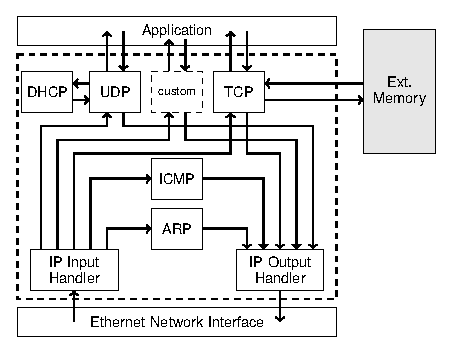
\includegraphics[scale=1]{introduction/fccm2015.eps}
\caption{The architecture of the Xilinx 10Gbps TCP/IP stack introduced in
\textit{Scalable 10Gbps TCP/IP Stack Architecture for Reconfigurable Hardware,
in FCCM’15}\cite{sidler2015tcp}.}
\label{fig:fccm2015}
\end{figure}

Fernando Lu{\'i}s Herrmann et al. have also created an UDP/IP network stack
in FPGA, achieving 1960 Mbps full-duplex throughput through their UDP/IP
network on a Spartan-3E XC3S500e-4FG320 FPGA\cite{Herrmann2009ANU}.\\
With a design able to both send and receive 8 bits per clock cycle, this
project was able to clock at $122.76 MHz$, limited by the IP transmitter, which
had the lowest speed. Interestingly, the whole system utilized only $14.19\%$
of the resources on the modest, and fairly outdated Xilinx Spartan 3E, with the
chip itself costing about $31.36$ USD at the time of writing\cite{XC3S500E}.





